\documentclass{endm}
\usepackage{endmmacro}
\usepackage{graphicx}
\usepackage[spanish]{babel}
\usepackage[utf8]{inputenc}



% The following is enclosed to allow easy detection of differences in
% ascii coding.
% Upper-case    A B C D E F G H I J K L M N O P Q R S T U V W X Y Z
% Lower-case    a b c d e f g h i j k l m n o p q r s t u v w x y z
% Digits        0 1 2 3 4 5 6 7 8 9
% Exclamation   !           Double quote "          Hash (number) #
% Dollar        $           Percent      %          Ampersand     &
% Acute accent             Left paren   (          Right paren   )
% Asterisk      *           Plus         +          Comma         ,
% Minus         -           Point        .          Solidus       /
% Colon         :           Semicolon    ;          Less than     <
% Equals        =           Greater than >          Question mark ?
% At            @           Left bracket [          Backslash     \
% Right bracket ]           Circumflex   ^          Underscore    _
% Grave accent  `           Left brace   {          Vertical bar  |
% Right brace   }           Tilde        ~

\newcommand{\Nat}{{\mathbb N}}
\newcommand{\Real}{{\mathbb R}}
\def\lastname{Colombo}

\begin{document}

% DO NOT REMOVE: Creates space for Elsevier logo, ScienceDirect logo
% and ENDM logo
\begin{verbatim}\end{verbatim}\vspace{2.5cm}

\begin{frontmatter}

\title{Hoy te convertís en (Junior) Data Scientist}

%\author{My Name\thanksref{ALL}\thanksref{myemail}}
\author{Ricardo Colombo}

%\address{My Department\\ My University\\ My City, My Country}
\address{Departamento de Computaci\on\\ Universidad de Buenos Aires\\ C.A.B.A, Argentina}

% \author{My Co-author\thanksref{coemail}}
% \address{My Co-authors Department\\ My Co-authors University\\
%    My Co-authors City, My Co-authors Country} \thanks[ALL]{Thanks
%    to everyone who should be thanked} \thanks[myemail]{Email:
%    \href{mailto:myuserid@mydept.myinst.myedu} {\texttt{\normalshape
%    myuserid@mydept.myinst.myedu}}} \thanks[coemail]{Email:
%    \href{mailto:couserid@codept.coinst.coedu} {\texttt{\normalshape
%    couserid@codept.coinst.coedu}}}

% \begin{abstract}
% This is a short example to show the basics of using the ENDM style
% macro files. Ample examples of how files should look may be found
% among the published volumes of the series at the ENDM home page
% ({\texttt{http://www.elsevier.com/locate/endm}})
% \end{abstract}

\begin{abstract}
El trabajo consiste en aplicar técnicas de Métodos numéricos y 
Data Science, en particular Regresiones Lineales y Cuadrados Mínimos, 
a un gran conjunto de datos reales, buscando identificar modelos 
capaces de predecir comportamientos.
\end{abstract}

\begin{keyword}
Data Science, KPIs, Cuadrados Minimos Lineales (CML)
\end{keyword}

\end{frontmatter}


\section{Introducción}\label{intro}

%Contendrá una breve explicación de la base teórica que fundamenta los métodos involucrados en el trabajo, junto con los métodos mismos. No deben incluirse demostraciones de propiedades ni teoremas, ejemplos innecesarios, ni definiciones elementales (como por ejemplo la de matriz simétrica). En vez de definiciones básicas es conveniente citar ejemplos de bibliografía adecuada. Una cita vale más que mil palabras

En la competitiva industria aeronáutica, la eficiencia de los procesos es vital para mantener la calidad del servicio. 
Cumplir con el servicio no es algo que solo dependa de la empresa que se contrata, ya que año a año la cantidad de vuelos se multiplica y muchas veces existen variables externas que terminen afectando la puntualidad y calidad del servicio. Por eso es importante contar con métricas que analicen los eventos pasados buscando patrones e intentar prevenirlos o disminuir su impacto en el futuro. Estos indicadores son denominados \textit{Key Performance Indicators} (KPIs).

Nuestro primer eje de estudio es la evolución en la cantidad de trafico aéreo de un aeropuerto, y como la cuota de \textit{market share} se fue concentrando con el correr del tiempo sobre las empresas líderes del segmento.

Nuestro segundo eje de estudio se centra en los factores estacionales que influyen en un vuelo salga en tiempo y forma, es decir estudiaremos la cantidad de retrasos en partidas para un aeropuerto particular, con el objetivo de detectar las estaciones anuales donde el clima pueda afectar el funcionamiento del aeropuerto.

Para la realización del trabajo analizaremos un set de datos reales correspondientes a vuelos realizados en Estados Unidos durante el periodo 2004 - 2008 dado a que no había datos para años anteriores a 2004 en relación a nuestras KPIs Luego buscaremos alguna relacion los ejes de estudio para estudiar si es posible predecir temporadas de mayor retraso debido al clima estimando la cantidad de vuelos.

\paragraph{Método de Mínimos Cuadrados}

Mínimos cuadrados es una técnica de análisis numérico, en la que, dados un conjunto de pares ordenados provenientes de un experimento intentaremos encontrar una relación entre los pares ordenados. Dado que estos valores poseen un error se intentara encontrar la función que mejor aproxime a los datos de acuerdo con el criterio de Error cuadrático medio. Intentaremos minimizar la suma de los cuadrados de las diferencias entre los puntos generados por la función de aproximación y los que corresponden a los datos.

\section{Desarrollo}

Para la simplificación del problema optamos por centrarnos en el aeropuerto \textit{JFK} y \textit{MIA} debido a que hoy día son dos de los aeropuertos que más movimiento presentan. Para el caso de \textit{JFK} sabemos que tiene estaciones invernales marcadas a fines de año que afectarían los vuelos ayudándonos en nuestros ejes de análisis

Como primer eje estudiaremos la evolución de la cantidad de vuelos de ese aeropuerto, entre dos de las empresas más reconocidas mundialmente \textit{Delta} y \textit{United Airlines}, Ambas con mayor presencia de vuelos. 

Luego como segundo eje estudiaremos la cantidad de demoras que se producen por condiciones climáticas. Tomando como definición de demora, un vuelo que sale al menos 15 minutos después de su horario programado, además que este tenga una demora debido al clima.
El objetivo de este caso es identificar temporadas cíclicas donde las condiciones climáticas afectan el comportamiento normal del aeropuerto. 

Para finalizar intentaremos probar si hay alguna relación la cantidad de vuelos y la cantidad de demoras estacionales generadas por el clima. Nuestra primera hipótesis que tenemos es que al aumentar el tráfico aéreo la demora por clima debería aumentar.

Para la realización del estudio implementamos una serie de algoritmos utilizando el lenguaje \textit{Python}. En la primer etapa procesamos el data set inicial filtrando algunos de los registros que nos interesa estudiar y los agrupamos por mes. Luego para entrenar nuestra solución propuesta tomamos un subconjunto de meses de los datos conocidos hasta encontrar el que nos de la mejor aproximación, ejecutamos el proceso para una cantidad \textit{k} tomando de a conjuntos de a k meses y validamos los resultados obtenidos utilizando la técnica de \textit{Coss-Validation}. Quedándonos con los que minimicen el error. Para evitar caer en el conocido overfitting elegiremos distintos subconjuntos del training para hallar los coeficientes de la aproximación lineal, para ambos entrenamientos usamos el periodo 2004-2007 para entrenamiento y test, luego realizamos una aproximación sobre el año 2008 y luego comparamos con los resultados reales, tanto la prediccion como lo que se uso para entrenamiento.

Luego el siguiente paso es ver como con los datos entrenados nuestras funciones que tan bien aproximan al valor real e intentar predecir el comportamiento futuro.

\section{Experimentacion y Resultados}
\subsection{Comparaci\on entre vuelos de Delta - American Airlines}
En primer lugar, para realizar este análisis debíamos cerciorarnos de las aerolíneas tomadas sean las más importantes para obtener un buen conjunto de datos y aplicar la técnica de CML. Para ello realizamos un gráfico con la cantidad de vuelos de cada una de las compañías con el mencionado fin.

\begin{center}
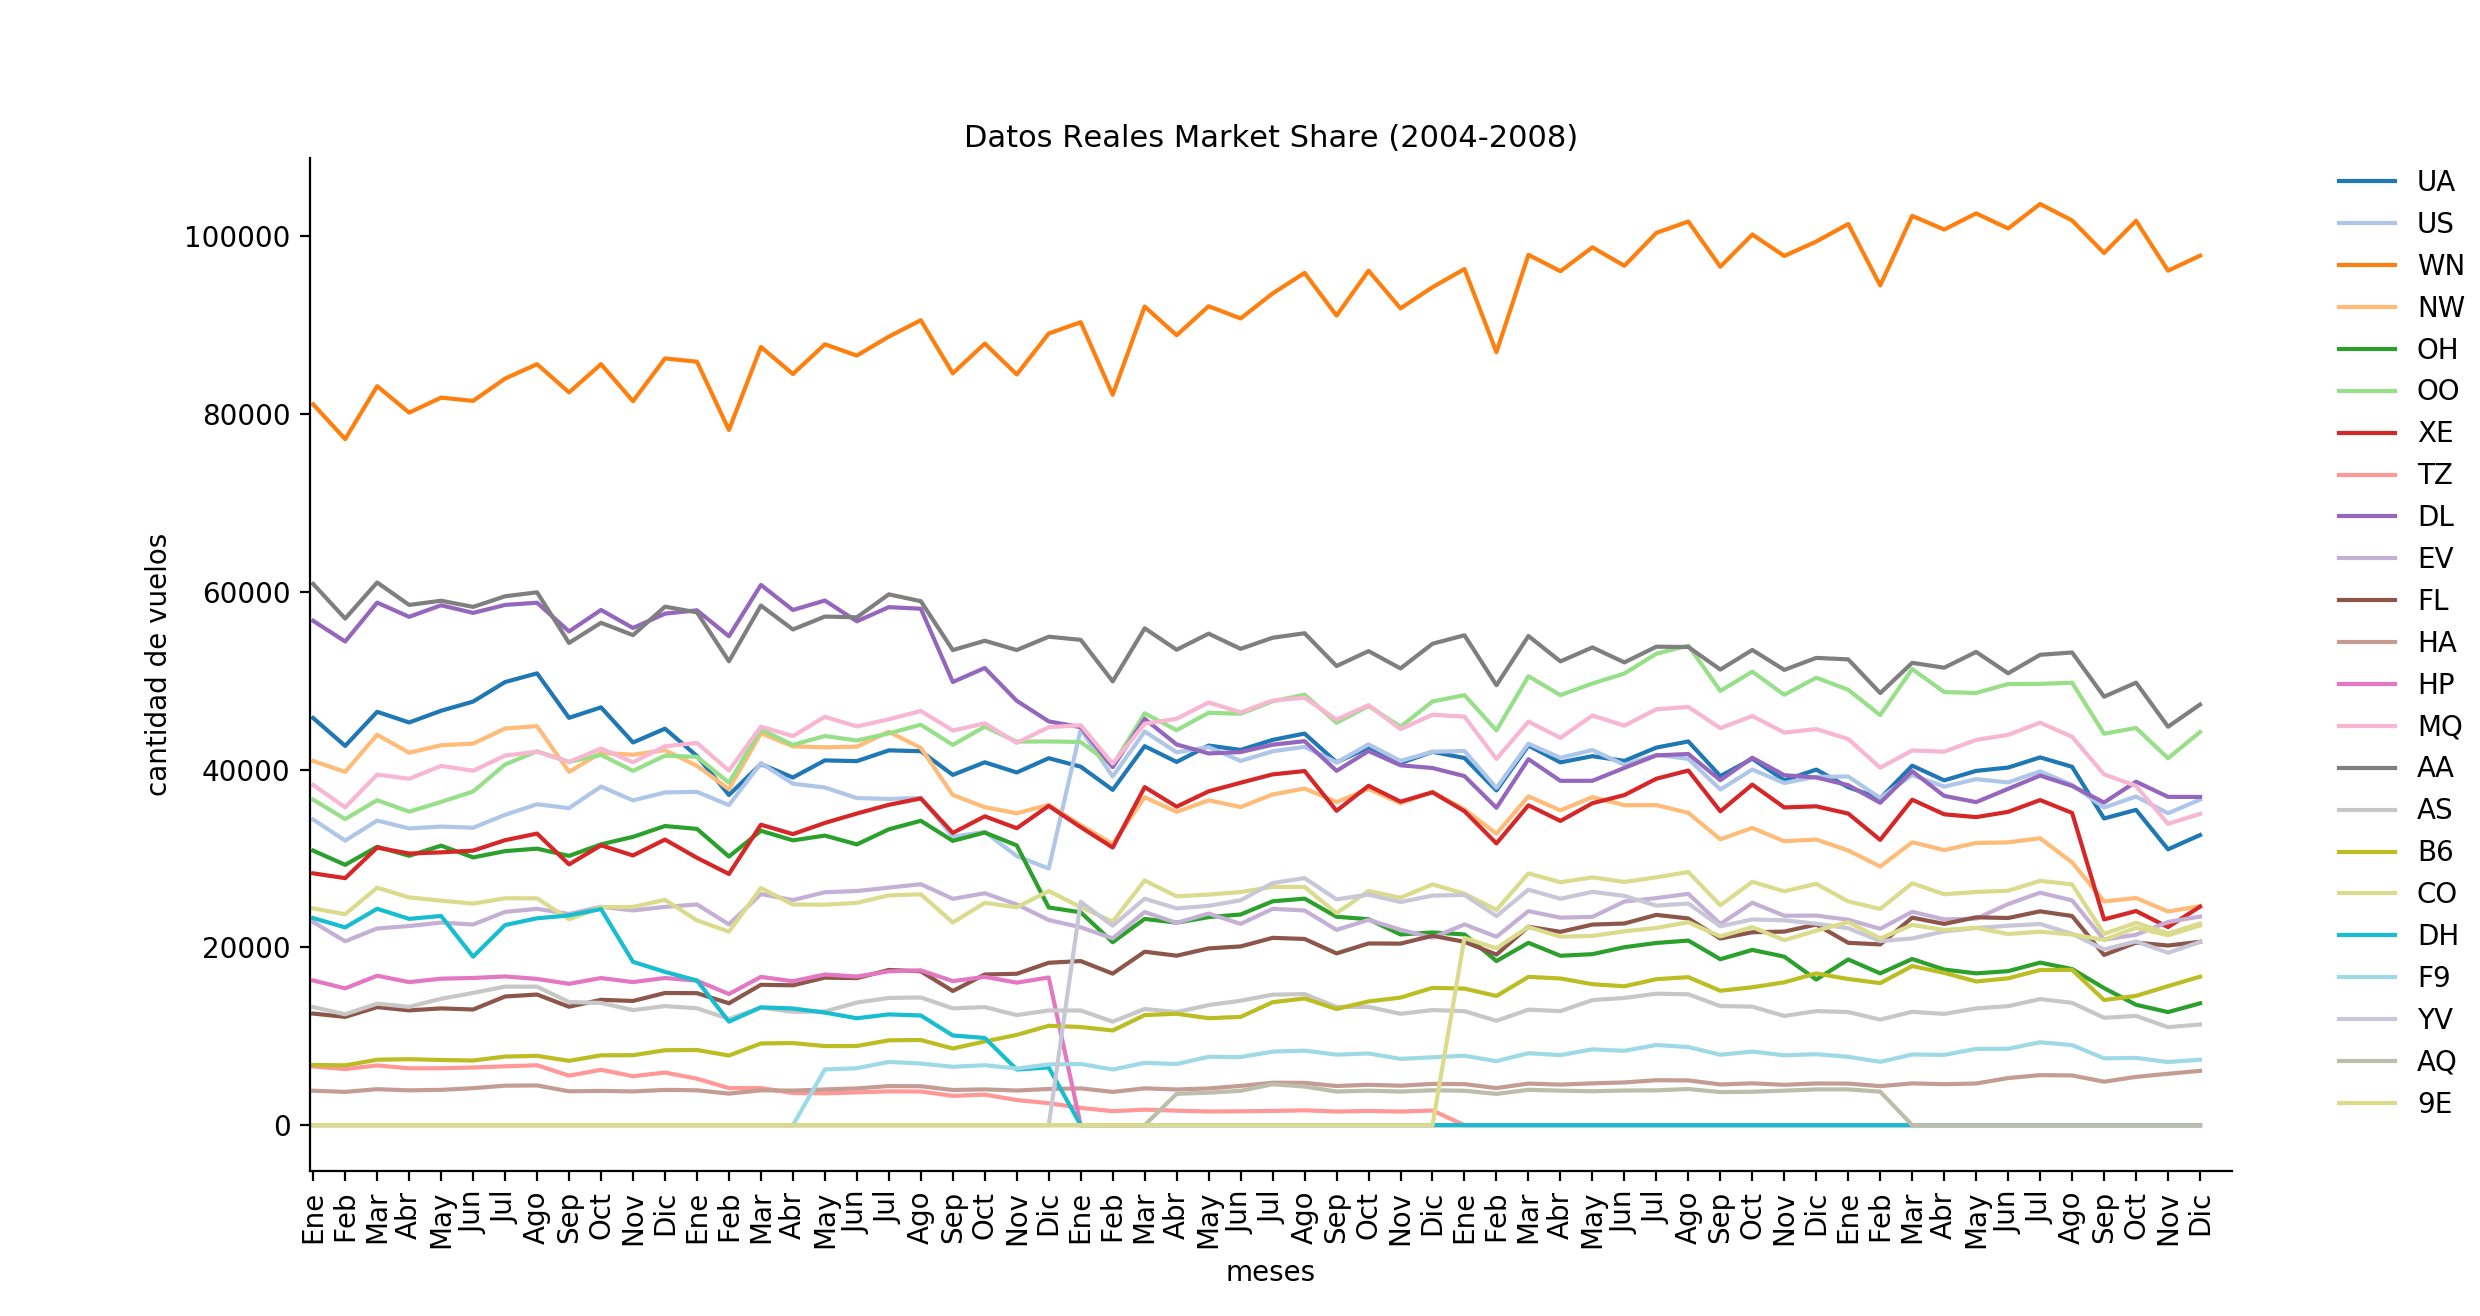
\includegraphics[scale=0.5]{imagenes/nuevas/MarketShare.png}
\end{center}

Como se puede observar, la aerolínea mas importante en cuanto a cantidad de vuelos totales, sin importar aeropuerto, es United Airlines (UA).

Para el resto de las aerolíneas es bastante parejo, lo que se puede notar a simple vista es que UA comienza a crecer mientras las demás tienen una leve baja en cuanto a cantidad de vuelos. Con esto podemos decir que se compensan en cierta forma los vuelos entre las compañías.

Por otro lado se nota que hay picos de caída en los vuelos para las fechas de Enero a Marzo, fechas de invierno en el hemisferio norte. A priori, ya tendríamos un indicador que para esas fechas tendríamos bajas de vuelos. No tiene ningún valor agregado en cuanto a las hipótesis respecto a los Delays.

Para este caso particular comenzamos analizando el aeropuerto de JFK. El cual nos arrojó la primera grafica en cuanto a Cantidad de vuelos.

\begin{center}
\includegraphics[scale=0.4]{imagenes/nuevas/vuelosDLJFK.png}
\end{center}

Para la construcción de nuestra predicción tomamos como set de entrenamiento los a\~nos 2005-2007 y realizamos una proyección sobre el año 2008, comparando los datos reales con la proyección obtenida por nuestra función. Esta elección se vio forzada a que la cantidad de vuelos crecía repentinamente entre 2004 y 2005 y afectaba la predicción considerablemente.
Luego de varios experimentos obtuvimos la siguiente aproximación.

\begin{center}
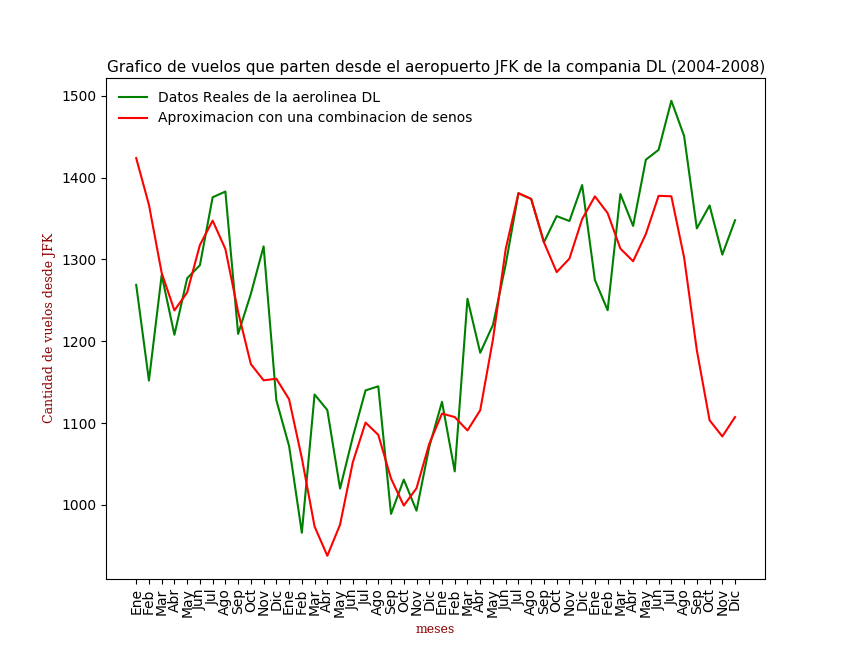
\includegraphics[scale=0.6]{imagenes/nuevas/DLCantSeno.png}
\end{center}

Como se puede observar la función decrece y crece a lo largo de los 3 años dándonos cierta periodicidad en ese periodo de 36 meses. Por otro lado tiene picos intermedios de cada año. Luego de experimentar vimos que la función que hacia mejor error sobre el set de datos fue la dada por:
$ a* cos(2* \pi *mes/36)+b*cos(2* \pi*mes/6)+c*sin(2*\pi*mes/11)+d$
Con a,b ,c y d los coeficientes de CML.

Luego Analizamos el caso de American Airlines de manera muy similar, la cual arrojo la siguiente grafica que nos llamó la atención y la explicamos a continuación de dicha imagen.

\begin{center}
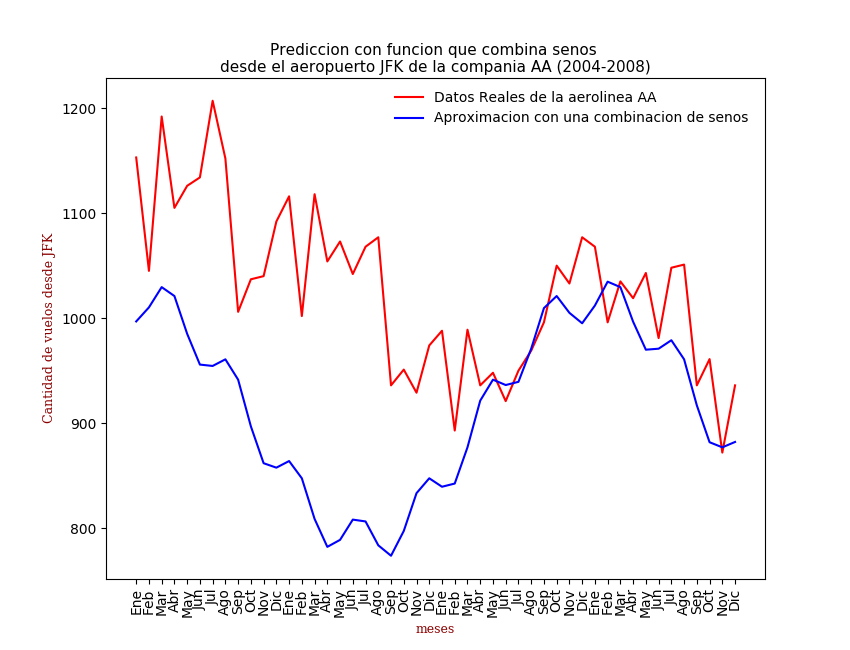
\includegraphics[scale=0.6]{imagenes/nuevas/AACantSeno.png}
\end{center}

Como se puede observar para los primeros años que se usaron para el cross validation, la función de aproximación acompaña en cierta forma a la real. Con esto queremos decir que cuando la función real decrece, la de prediccion tambien y analogo cuando crece.Pero lo más llamativo acá fue que la predicción para 2008 ( ultimo año ) fue bastante acertada.

Cabe destacar que esta función no solo pareciera tener periodicidad al igual que la anterior, donde su ciclo completo pareciera ser al año, si no que posee un cambio con los datos como se ver reflejada en el centro de la misma. De igual manera, CML aproximo bien cuando se utilizó cross validation para k=4.

Para esta aerolínea la función que hacia mejor aproximo fue:
$ a* cos(2* \pi *mes/36)+b*cos(2* \pi*mes/5)+c*sin(2*\pi*mes/5)+d$
Con a,b ,c y d los coeficientes de CML.

Por último, probamos con el aeropuerto de MIA (Miami), para analizar otro conjunto de datos el cual. Dado la ubicación geográfica y la gran demanda anual de vuelos que tiene por ser un lugar que tiene vuelos durante todo el año, aplicamos las técnicas para hacer la predicción.

\begin{center}
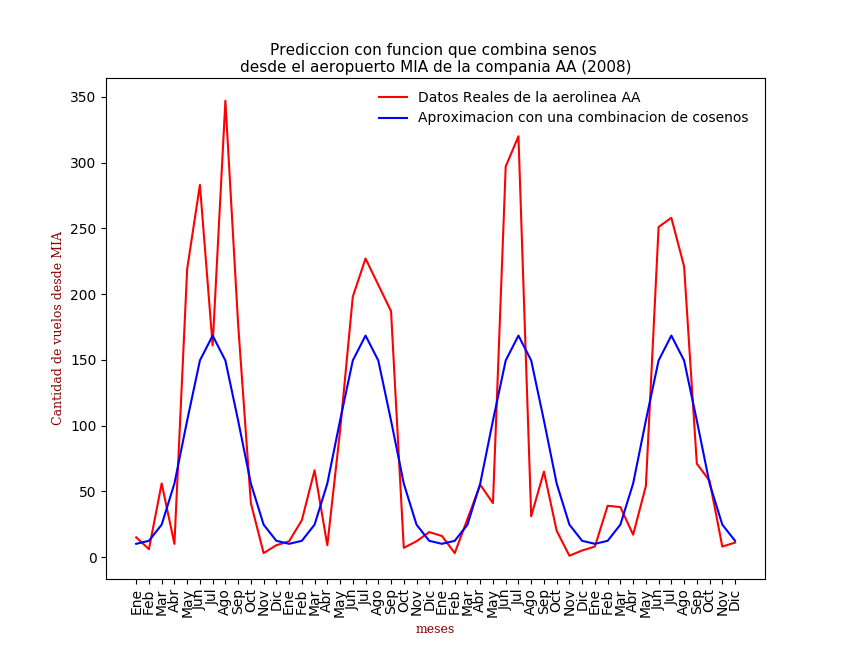
\includegraphics[scale=0.6]{imagenes/nuevas/AAMIACantSeno.png}
\end{center}
 La cual es una función con una periodicidad más marcada, la cual permite ser mejor aproximada con el uso de funciones trigonométricas. Mas puntualmente con senos.

A continuación, mostraremos algunos de los errores que fue arrojando CML para los distintos valores de los coeficientes donde el valor minimo fue el utilizado, con el fin de dar una métrica de cuál es el que se está utilizando en cada uno de los gráficos de cantidad de vuelos en AA y DL en JFK. 
\begin{center}
    \begin{tabular}{| 1 | 1 | 1 | 1 | 1 |}
    \hline
    a & b & c & d & error \\ \hline
 526.97978103 & -22.4643293   &-22.4643293  & 620.89645918  &2723407.25\\
 -176.72792282  &  12.52220812  &  12.52220812 & 1249.13176871 &652275.25\\
 -188.7948473  &   -7.90368338  &  -7.90368338 & 1030.8041969 & 277589.0\\
  737.96822254 &   64.50296201 &   64.50296201 & 1594.40541198& 5226845.5\\
 454.50182561  & -8.88598173  & -8.88598173 & 633.51012576& 2329134.5\\
    \hline
    \end{tabular}
\end{center}
\begin{center}
    \begin{tabular}{| 1 | 1 | 1 | 1 | 1 |}
    \hline
    a & b & c & d & error \\ \hline
-542.14932626  &257.23799748 &-207.9280451  & 706.30852002& 6608977.66667\\
 -987.65817544 & -237.70338425&  -596.35771535 & 1412.34035509 &10853930.3333\\
  134.36765167  &  73.18658559  &  46.0117051   &1246.22359027 &160404.666667\\
  179.50199147  &  57.67834695 &  -47.28161852 & 1186.77029749 &79742.3333333\\
 689.71618516  & 78.41594853& -177.59932851  &834.10421078& 3545511.0\\
    \hline
    \end{tabular}
\end{center}

\section{Demoras Climáticas}
Para este eje, utilizamos el aeropuerto de JFK (New York) . El fin de esto es ver dos puntos con gran cantidad de datos para observar los movimientos y dado a su posición Geográfica tiene estaciones marcadas con nevadas que perjudican los vuelos,queremos ver ademas si hay algun tipo de conexión con el otro eje de estudio.

Al igual que en el caso anterior, previamente analizamos ambas gráficas y utilizamos Cross validaton en conjunto con CML para aproximar las funciones las cuales dieron las siguientes gráficas.

Para el caso de JFK:
\begin{center}
\includegraphics[scale=0.3]{imagenes/nuevas/DelaySeno.png}
\end{center}

Como se pueden ver los picos de delays tienen cierta periodicidad, esto a priori nos indicaría que podíamos utilizar las funciones trigonométricas porque comparten esta característica. 
Estos Delays se producen con mayor frecuencia en Diciembre a marzo, resulta esperable para ser invierno, y en Mayo a Octubre. Finalmente podemos ver que la cantidad de vuelos es menor y la cantidad de delays por clima es mayor para esa época, confirmando nuestra hipótesis en relación a ambos ejes.
Luego de varias pruebas la que mejor aproximo fue la que esta presentada con la función de aproximación $a* sin(2*\pi*mes/12)+b*cos(2*\pi*mes/6)+c*sin(2*\pi*mes/8)+d$ siendo a,b,c y d los coeficientes calculados por CML.

\section{Conclusiones}
	%Hablar sobre la función final que escogimos y como reúne los que queremos de la dos funciones

Luego de analizar los resultados obtenidos vemos que las funciones propuestas acompañan a la función de datos reales, pero tratar de proyectar los \textit{Key Performance Indicators} que se están estudiando para un futuro de mediano plazo puede resultar en una predicción no muy certera. Ya que no hay forma de tener en consideración factores externos que generen un outlier sobre los datos reales. Por ejemplo un pico de venta mensual o un invierno con tormentas de nieve que no son muy predecibles.

Por otro lado notamos que las funciones trigonométricas resultan ser buenas al momento de aproximar, con esto podemos confirmar que de igual manera está atado a la función de aproximación que se utiliza.

\section{Apéndice}
Archivos usados en este informe, normalmente salvan directamente la imagen en la carpeta src.
\begin{itemize}
\item jfkdl.py , jfkaa.py , marketshare.py ,miaaa.py Sección comparación compañías
\item main.py - sección clima 
\end{itemize}
\begin{thebibliography}{10}\label{bibliography}
  
\bibitem{bf} Burden, R. L., and J. D. Faires, ``Análisis numérico,
 Math. Surveys \textbf{7}, Amer. Math. Soc.,
  Providence, R.I., 1961.
  
\bibitem{d} ASA Section on Statistical Computing. 2009 data expor competition, URL:
  \href{http://stat-computing.org/dataexpo/2009/the-data.html}
  {\texttt{http://stat-computing.org/dataexpo/2009/the-data.html}}.

\end{thebibliography}

\end{document}